%; whizzy chapter
% -initex iniptex -latex platex -format platex -bibtex jbibtex -fmt fmt
% 以上 whizzytex を使用する場合の設定。

%     Tokyo Debian Meeting resources
%     Copyright (C) 2011 Junichi Uekawa
%     Copyright (C) 2011 Nobuhiro Iwamatsu

%     This program is free software; you can redistribute it and/or modify
%     it under the terms of the GNU General Public License as published by
%     the Free Software Foundation; either version 2 of the License, or
%     (at your option) any later version.

%     This program is distributed in the hope that it will be useful,
%     but WITHOUT ANY WARRANTY; without even the implied warranty of
%     MERCHANTABILITY or FITNESS FOR A PARTICULAR PURPOSE.  See the
%     GNU General Public License for more details.

%     You should have received a copy of the GNU General Public License
%     along with this program; if not, write to the Free Software
%     Foundation, Inc., 51 Franklin St, Fifth Floor, Boston, MA  02110-1301 USA

%  preview (shell-command (concat "evince " (replace-regexp-in-string "tex$" "pdf"(buffer-file-name)) "&"))
% 画像ファイルを処理するためにはebbを利用してboundingboxを作成。
%(shell-command "cd image201101; ebb *.png")

%%ここからヘッダ開始。

\documentclass[mingoth,a4paper]{jsarticle}
\usepackage{monthlyreport}

% 日付を定義する、毎月変わります。
\newcommand{\debmtgyear}{2011}
\newcommand{\debmtgmonth}{5}
\newcommand{\debmtgdate}{21}
% (+ (* (- 2010 2005) 12) 10) started from zero
\newcommand{\debmtgnumber}{76}

\begin{document}

\begin{titlepage}
\thispagestyle{empty}
% タイトルページ:編集必要な部分は最初のマクロに飛ばすこと

\vspace*{-2cm}
第\debmtgnumber{}回 東京エリア Debian 勉強会資料\\
\hspace*{-2cm}

\includegraphics[width=210mm]{image201003/debsen.eps}\\
\hfill{}\debmtgyear{}年\debmtgmonth{}月\debmtgdate{}日

% ここはアップデートすること
\rotatebox{10}{\fontsize{32}{32} {\gt 特集1: Apache2 モジュールを作ってみた}}

\rotatebox{10}{\fontsize{32}{32} {\gt 特集2: Debian/m68k 開発}}

\vspace*{-2cm}
\hfill{}
\includegraphics[height=6cm]{image200502/openlogo-nd.eps}
\end{titlepage}

\dancersection{Introduction}{上川 純一}

\begin{multicols}{2}
 

 今月のDebian勉強会へようこそ。これからDebianの世界にあしを踏み入れると
 いう方も、すでにどっぷりとつかっているという方も、月に一回Debianについ
 て語りませんか?

 Debian勉強会の目的は下記です。

 \begin{itemize}
 \item \underline{Debian Developer} (開発者)の育成。
 \item 日本語での「\underline{開発に関する情報}」を整理してまとめ、アップデートする。
 \item \underline{場}の提供。
 \begin{itemize}
  \item 普段ばらばらな場所にいる人々が face-to-face で出会える場を提供
	する。
  \item Debian のためになることを語る場を提供する。
  \item Debianについて語る場を提供する。
 \end{itemize}
 \end{itemize}		

 Debianの勉強会ということで究極的には参加者全員がDebian Packageをがりがり
 と作るスーパーハッカーになった姿を妄想しています。情報の共有・活用を通し
 て Debianの今後の能動的な展開への土台として、「場」としての空間を提供す
 るのが目的です。

\end{multicols}

\newpage

\begin{minipage}[b]{0.2\hsize}
 \definecolor{titleback}{gray}{0.9}
 \colorbox{titleback}{\rotatebox{90}{\fontsize{80}{80} {\gt デビアン勉強会} }}
\end{minipage}
\begin{minipage}[b]{0.8\hsize}
\hrule
\vspace{2mm}
\hrule
\begin{multicols}{2}
\tableofcontents
\end{multicols}
\vspace{2mm}
\hrule
\end{minipage}

\dancersection{事前課題}{岩松 信洋}

今回の事前課題は以下です:
\begin{enumerate}
 \item Debian使いとしてウェブサービスに期待することは何ですか?
\end{enumerate}
この課題に対して提出いただいた内容は以下です。
\begin{multicols}{2}
{\small
%; whizzy-master ../debianmeetingresume201101.tex
% $B0J>e$N@_Dj$r$7$F$$$k$?$a!"$3$N%U%!%$%k$G(B M-x whizzytex $B$9$k$H!"(Bwhizzytex$B$,MxMQ$G$-$^$9!#(B



\begin{prework}{ $B%-%?%O%i(B }

Debian$B8BDj$@$H;W$$$D$+$J$$!&!&!&!#(B
($B$*Bj$N0U?^$rFI$_0c$($F$$$k$N$+$b(B)
apt-get$B$r(Bhttp$B$G<B9T$9$k$H%&%'%V%5!<%S%9$H8@$($k(B?
\end{prework}

\begin{prework}{ MATOHARA }

Debian$B;H$$$H$7$F%&%'%V%5!<%S%9$K4|BT$9$k$3$H!%(B
$B:G6a$O>/$J$/$J$j$^$7$?$,!$(BIE $BI,?\$N%5!<%S%9Ey$N4D6-0MB8$N%5!<%S%9$r$d$a(B
 $B$FM_$7$$$G$9!%(B
$B:G6a$@$H(BSilverlight $BI,?\$N%5!<%S%9$G(BMoonlight $B$GF0$-$=$&$GF0$+$J$$$H$$$C(B
 $B$?$3$H$,$"$j$^$7$?!%(B
\url{http://live6.channel.ne.jp/world_ipv6/}
\end{prework}

\begin{prework}{ taitioooo }

$B>pJs$KBP$9$k2]6b$,$J$/$J$k$3$H!#(B

\end{prework}

\begin{prework}{ $BLnEg!!5.1Q(B }

\begin{itemize}
\item jslinux$B$H$$$&6/NO$J%(%_%e%l!<%?$b=P$?$N$G!"%V%i%&%6$GF0$/(BDebian
 experimental$B4D6-$H$+%V%i%&%6$GF0$/(BGnome$B$N$*;n$74D6-$H$+$rDs6!$9$k%&%'%V(B
 $B%5!<%S%9$H$+AGE($+$b!#(B
$B$3$b$-$C$H%&%'%V%5!<%S%9!*!J$J$s$+6u5$FI$a$F$J$$2sEz$J5$$b$9$k$1$I(B...)

\item USB$B$K=q$-9~$a$P(Bdebian$B4D6-$,$=$N$^$^%V!<%H$G$-$k$h$&$J%$%a!<%8$r$D$/$C$F(B
 $B$/$l$k%&%'%V%5!<%S%9$,NI$5$=$&$J5$$b(B...$BNc$($P!"%Q%C%1!<%80lMw$K%A%'%C%/(B
 $BF~$l$F!"(Bsid$B$H$+$K%A%'%C%/F~$l$k$H!"(BUSB$B%a%b%j$K$=$N$^$^=q$-9~$a$P$=$N;E(B
 $BMM$G(Bdebian sid$B$,%V!<%H$G$-$k$h$&$J%+%9%?%`%$%a!<%8$r:n$C$F$/$l$k$H$+!#(B

\item $B%A%'%C%/%\%C%/%9$H%;%l%/%?$@$1$G!"(Bpreceed$B%U%!%$%k@8@.$7$F$/$l$k%&%'%V%5!<(B
 $B%S%9$b$$$$$+$b(B...$BBgNL$N%$%s%9%H!<%k;~$H$+$h$5$=$&!#(B
$B!J$b$&8@$$$?$$J|Bj$G$9$M(B...)
\end{itemize}











\end{prework}

\begin{prework}{ $B4d>>(B $B?.MN(B }
\begin{itemize}
\item $BA4@$3&$N(BWeb$B%5!<%P$rDs6!$9$k(BOS$B$,(BDebian$B$K$J$k$3$H!#(B
\item $BJ,;6%3%s%Q%$%k%5!<%P$H$+M_$7$$!#(B
\end{itemize}


\end{prework}

\begin{prework}{ $BF|HfLn(B $B7<(B }

Web$B%5!<%S%9$b$G$-$l$P5!3#=hM}$7$d$9$$$b$N$,NI$$!#(B
$B$"$H!"%/%i%&%I>e$G$N(BAPI$B$rDs6!$7$F$$$k$h$&$J%5!<%S%9$K!"4X?t7?8@8l$KBP$9(B
 $B$k%5%]!<%H$,A}$($F$[$7$$!#(B

\end{prework}

\begin{prework}{ dictoss($B?yK\!!E5=<(B) }

CPU$B$H$"$k(Bdeb$B%Q%C%1!<%8$rA*Br$9$k$H!"$=$N(BCPU$B8~$1$K:GBg8B$N:GE,2=$7$?%Q%C(B
 $B%1!<%8$H0MB8$9$k%Q%C%1!<%8$r:F%S%k%I$7$F$/$l$k%5!<%S%9!#(B
\end{prework}

\begin{prework}{ kazken3 }

$BK]Lu$r$?$^$K$7$F$$$k$N$G!"%G%#%9%H%j%S%e!<%7%g%s4V2#$I$*$7$G$NK]Lu4XO">p(B
 $BJs$rDs6!$9$k%5%$%H$,$"$l$P$$$$$J$H;W$&$3$H$,$"$j$^$9!#(B

$B!t2]Bj$H$O>/$7%:%l$F$$$k$+$bCN$l$^$;$s$,!"(B
$B!t8D?M8~$1$N%&%'%V%5!<%S%9$K$O?)=}5$L#$H$$$&$H$3$m$b$"$k$N$G!#(B


\end{prework}

\begin{prework}{ $B$^$($@$3$&$X$$(B }

Debian$B%7%9%F%`$G:n$C$?4D6-$H$NAj8_8_49@-!#(B
$BNc$($P!":G6a(BGAE/Python$B$r$h$/;H$&$N$G!":n$C$?%7%9%F%`$r(B
 GAE/Python <-> $B"*(BDebian$B%7%9%F%`$N$I$A$i$G$b(B($B$[$H$s$IJQ99$J$7$G(B)$BF0$+$;$k$H(B
 $BJXMx$G$9$M!#(B
$B$9$0;O$a$k$N$K%/%i%&%I%5!<%S%9$rMxMQ$7$F:n$C$?$1$I>-Mh$O(BDebian$B$GF0$+$7$?(B
 $B$$!"5U$K:#$O@/<#E*$JM}M3$G30$K=P$;$J$$(BDebian$B%7%9%F%`$r>-Mh$O<+J,$N4IM}(B
 $B$+$i30$l$k$N$G<jN%$l$r$h$/$9$k$?$a$K%/%i%&%I%5!<%S%9$K4JC1$K0\9T$G$-$k!"(B
 $B$J$I!#(B
\end{prework}

\begin{prework}{ yamamoto }

$B$=$&$G$9$M!#(B
$B:#$N=jF3F~$r8!F$$7$F$$$k$N$O!"%Q!<%=%J%k%9%H%l!<%8%5!<%S%9$0$i$$$G$9$+$M!#(B
$B$"$i$f$k=j$G<+J,$N%G!<%?$,<+J,$G6&M-$G$-$l$P!"$=$l$G==J,$J46$8$G$9!#(B
\end{prework}

}
\end{multicols}

\dancersection{最近のDebian関連のミーティング報告}{岩松 信洋}
\subsection{東京エリアDebian勉強会75回目報告}

% (query-replace-regexp "<.*?>" "")
% (query-replace-regexp "^[	 ]\+" "")



\dancersection{Debian Trivia Quiz}{岩松 信洋}

ところで、みなさん Debian 関連の話題においついていますか?Debian関連の話
題はメーリングリストをよんでいると追跡できます。ただよんでいるだけではは
りあいがないので、理解度のテストをします。特に一人だけでは意味がわからな
いところもあるかも知れません。みんなで一緒に読んでみましょう。

今回の出題範囲は\url{debian-devel-announce@lists.debian.org} や \url{debian-devel@lists.debian.org}に投稿された
内容とDebian Project Newsからです。

\begin{multicols}{2}
% %; whizzy-master ../debianmeetingresume201101.tex
% $B0J>e$N@_Dj$r$7$F$$$k$?$a!"$3$N%U%!%$%k$G(B M-x whizzytex $B$9$k$H!"(Bwhizzytex$B$,MxMQ$G$-$^$9!#(B
%
% $B$A$J$_$K!"%/%$%:$OJL%V%i%s%A$G:n@.$7!"$N$A$K%^!<%8$7$^$9!#5U$K%^!<%8$7(B
% $B$J$$$h$&$K$7$^$7$g$&!#(B
% (shell-command "git checkout quiz-prepare")

\santaku
{RC$B%P%0$N8=>u$O$O$I$3$G3NG'$G$-$k$+(B}
{\url{http://bugs.debian.org/release-critical/}}
{\url{http://localhost/}}
{\url{http://debianmeeting.appspot.com/}}
{A}

\santaku
{Debian$BJY6/2qM=Ls%7%9%F%`$N(BURL$B$O$I$l$+(B}
{\url{http://www.2ch.net/}}
{\url{http://atnd.org/events/}}
{\url{http://debianmeeting.appspot.com/}}
{C}

\santaku
{events@debian.org$B$O$I$3$HE}9g$5$l$?$+(B}
{merchants@debian.org}
{hoge@debian.org}
{fuga@debin.org}
{A}

\santaku
{antiharassment@debian.org $B$N$&$i$K$$$J$$$N$OC/$+(B}
{Amaya Rodrigo Sastre}
{Patty Langasek}
{Kouhei Maeda}
{C}

\santaku
{Sprint$B$G$O$J$$$N$O$I$l$+(B}
{-www sprint}
{security sprint}
{tokyo sprint}
{C}

\santaku
{DACA$B$O$I$3$r8+$l$P$h$$$+(B}
{\url{http://qa.debian.org/daca/}}
{\url{http://daca.debian.org/}}
{\url{file:/tmp}}
{A}

\santaku
{DEP $B$O2?$NN,$+(B}
{Debian Enhancement Proposal}
{Device Enhancement Protocol}
{$B$G$C$W(B}
{A}

\santaku
{DEP5$B$GDs0F$5$l$F$$$k(Bdebian/copyright$B$N5!3#2DFI7A<0$O$I$&$$$&$b$N$+(B}
{S$B<0(B}
{RFC822$BIw(B}
{XML}
{B}


\end{multicols}

%-------------------------------------------------------------------------------
\dancersection{Apache2 のモジュールをつくってみた}{上川純一}
%-------------------------------------------------------------------------------
\index{apache}

Apache httpd というウェブサーバがあります。おそらく定番と言われるウェブ
サーバで、多くの人が利用していると思います。ウェブサーバとして多くの機能
を提供しているApacheですが、モジュールという仕組みで機能拡張可能です。
今回はDebian上でApacheモジュールを作る方法をさぐってみることにします。

\subsection{Apacheモジュールをつくりたいとき}

Apacheモジュールが作りたいときはどういうときでしょうか。作りたいと思った
ときがつくりどき。cgiでfork する手間が惜しい、インタプリタ言語でインタプ
リタが走っている時間がもったいない、GCのある言語でときどき反応が悪くなる
のが気にくわない。いろんな理由があるとおもいますが、C言語でがりがりとウェ
ブリクエストを処理したいとかそういう要望があるのではないでしょうか。

Apacheモジュールでできることはどういうことでしょうか。Apacheの受け取る入
力(HTTP Request)から出力(HTTP Response)のほぼ任意の場所にフックとして割り
込むことができて、入出力のデータを加工することが可能です。

\subsection{Debian の Apache パッケージの構成}

ところで、httpd と Debian apache2 はどれくらい違うかご存知でしょうか。

Debian パッケージのREADME.Debian を見てみましょう。
\cite{Apache2ReadmeDebian}

ざっと眺めただけでも以下の点で特徴があります。

\begin{itemize}
 \item  apache2コマンドが環境変数に依存している。
 \item  apache2ctl / /etc/init.d/apache2 を利用しないと起動とかできない。
 \item  設定ファイルの配置が全然違う。
 \item  a2enmod / a2dismod コマンドが追加されている。
 \item  apxs コマンドが apxs2 という名前になっている。
\end{itemize}

\subsection{Apacheモジュールの作成}

普通のApacheモジュールの作成の流れをみてみましょう。

\subsubsection{パッケージの準備}

とりあえず開発環境をインストールしましょう。
\begin{commandline}
# apt-get install apache2-threaded-dev
\end{commandline}

\subsubsection{テンプレート生成}

apxs2 コマンドを利用してテンプレートを作成します。
モジュール名でディレクトリが作成されます。
\index{apxs2}

\begin{commandline}
$ apxs2 -g -n dancerqps
$ cd dancerqps
$ ls 
$ ls
Makefile  mod_dancerqps.c  modules.mk
\end{commandline}

\subsubsection{ソースコード編集}

ソースコードを編集しましょう。この場合、自動で生成された
\url{mod_dancerqps.c}がメインのモジュールソースコードです。

まず一番下に一番重要な構造が定義されています。ここで重要なのは
\verb!dancerqps_register_hooks! を登録しているところでしょうか。

\begin{commandline}
module AP_MODULE_DECLARE_DATA dancerqps_module = {
    STANDARD20_MODULE_STUFF,
    NULL,                  /* create per-dir    config structures */
    NULL,                  /* merge  per-dir    config structures */
    NULL,                  /* create per-server config structures */
    NULL,                  /* merge  per-server config structures */
    NULL,                  /* table of config file commands       */
    dancerqps_register_hooks  /* register hooks                      */
};
\end{commandline}


\verb!dancerqps_register_hooks!で実際にフックの登録を行います。
ここでは、アウトプットフィルタを登録しています。
\begin{commandline}
static void dancerqps_register_hooks(apr_pool_t *p) {
  ap_register_output_filter(dancerqps_name, dancerqps_filter,
			    NULL, AP_FTYPE_RESOURCE);
}
\end{commandline}

そして、実際に各リクエストのアウトプットに対して実効するフィルタのコード
を書きます。

\begin{commandline}
static apr_status_t dancerqps_filter(ap_filter_t *f, apr_bucket_brigade *bb) {
  /* ここでなにか処理をする */
  ap_log_rerror(APLOG_MARK, APLOG_ERR, 0, f->r,
		"dancerqps processing was here!");
  return ap_pass_brigade(f->next, bb);
}
\end{commandline}

\subsubsection{モジュールのファイルインストール}

モジュールをビルドしてインストールする一連の手順をしてくれるコマンドがあ
ります。

\begin{commandline}
$ sudo apxs2 -c -i mod_dancerqps.c
\end{commandline}

\subsubsection{モジュールを有効にする}

apxs2 コマンドでモジュールを有効にする方法は Debian独自のa2enmodなどのコマンドの存在
を無視しているようなのでa2enmodなどと整合性のとれるような方法をとるのが
よいでしょう。
で、それではDebian的な方法とはなんでしょうか。

\subsubsubsection{Debian way 1}

めんどくさい方法だけどシステム運用者としては便利かもしれない方法。
a2enmodとかができます。

/etc/apache2/mods-available に hoge.conf, hoge.load ファイルを作成します。
hoge.conf は設定が不要なら不要ですが、httpd.confに書くような内容を記述し
ます。
hoge.load には LoadModule行を記述します。

この方法でファイルを作成しておけば、/etc/apache2/mods-enabledディレクト
リにシンボリックリンクが作成されます。

\subsubsubsection{Debian way 2}

デフォルトでは空のファイルだけど、/etc/apache2/httpd.conf に書き込むとそ
の設定が有効になります。

\begin{commandline}
LoadModule test_module /usr/lib/apache2/modules/mod_test.so
<Location "/hoge/">
   SetHandler test
</Location>
\end{commandline}

\subsubsubsection{Debian的な方法から乖離しているっぽい方法}

apache をコマンドラインから設定ファイルを指定して起動することができます。
DebianのApacheは環境変数を設定しないと直接は起動できなくなっているので、
面倒な手続きが必要になります。

まず、適当にテスト用のhttp.confをでっち上げます。

\begin{commandline}
Listen 8080

LockFile /home/test/tmp/apache.1.lock
PidFile /home/test/tmp/apache.1.pid

# log configuration.
LogFormat "%h %l %u %t \"%r\" %>s %b" common
CustomLog "/home/test/log/access_log" common
ErrorLog "/home/test/log/error_log"

# Order, Allow.
LoadModule authz_host_module /usr/lib/apache2/modules/mod_authz_host.so
# map from / -> /index.html
LoadModule dir_module /usr/lib/apache2/modules/mod_dir.so
DirectoryIndex index.html index.cgi index.pl index.php index.xhtml index.htm
# .html -> content-type: text/html
LoadModule mime_module /usr/lib/apache2/modules/mod_mime.so
TypesConfig /etc/mime.types

# Document root
DocumentRoot "/home/test/hoge"
<Directory "/home/test/hoge">
    Options Indexes FollowSymLinks

    AllowOverride None

    Order allow,deny
    Allow from all

</Directory>

# Load my custom filter.
LoadModule dancerqps_module /usr/lib/apache2/modules/mod_dancerqps.so
SetOutputFilter DANCERQPS
\end{commandline}

適当な設定ファイルを指定してApacheを起動してみます。

\begin{commandline}
APACHE_RUN_USER=dancer \
 APACHE_RUN_GROUP=dancer \
 /usr/sbin/apache2 -f $(readlink -f ./httpd.conf) -k restart 
\end{commandline}
% $

\subsubsection{負荷テスト}
\index{ab}

ab (apachebench) ツールが標準で入っているのでそれで計測します。適当に確
認しましょう。

\begin{commandline}
$ /usr/sbin/ab -c 100 -n 100 http://localhost:8080/ 
This is ApacheBench, Version 2.3 <$Revision: 655654 $>
Copyright 1996 Adam Twiss, Zeus Technology Ltd, http://www.zeustech.net/
Licensed to The Apache Software Foundation, http://www.apache.org/

Benchmarking localhost (be patient).....done


Server Software:        Apache/2.2.9
Server Hostname:        localhost
Server Port:            8080

Document Path:          /
Document Length:        44 bytes

Concurrency Level:      100
Time taken for tests:   0.056 seconds
Complete requests:      100
Failed requests:        0
Write errors:           0
Total transferred:      29600 bytes
HTML transferred:       4400 bytes
Requests per second:    1796.17 [#/sec] (mean)
Time per request:       55.674 [ms] (mean)
Time per request:       0.557 [ms] (mean, across all concurrent requests)
Transfer rate:          519.21 [Kbytes/sec] received

Connection Times (ms)
              min  mean[+/-sd] median   max
Connect:        7    9   0.5      9      10
Processing:     9   26   8.9     27      40
Waiting:        6   26   9.3     27      40
Total:         16   36   8.9     37      49

Percentage of the requests served within a certain time (ms)
  50%     37
  66%     41
  75%     43
  80%     45
  90%     47
  95%     48
  98%     49
  99%     49
 100%     49 (longest request)
\end{commandline}

\subsubsection{まとめ}

はじめてApacheモジュールを作成して、インストールして動かすところまでやっ
てみました。


\begin{thebibliography}{}
 \bibitem{Apache2ReadmeDebian} \url{/usr/share/doc/apache2.2-common/README.Debian.gz}
\end{thebibliography}


%-------------------------------------------------------------------------------
\dancersection{Debian/m68k 開発}{岩松 信洋}
%-------------------------------------------------------------------------------
\index{m68k}

Debian/m68k 開発環境を構築する機会があったのでまとめてみました。

\subsection{m68k とは?}
m68k とはなにか?Motorola 680x0/m68000/68000 の事。
省略してm68k。
32bit で CISC。エンディアンはビッグ。
世界中で未だに人気にあるCPUの一つ。
今はフリースケール・セミコンダクタによって、
Coldfireという名前で製造および販売されています。
なので今は68kと言うことが多いです(モトローラじゃないから)。
Apple社のMacintosh SEやシャープのX68000、Palm PilotのCPUとして活躍していました。
もちろん Linuxでもサポートされており、Debian では hamm から正式にサポート
アーキテクチャとして採用されましたが、etch から脱落しました。
Debian に最初にポーティングされ、最初に脱落したアーキテクチャということ
で覚えておくと良いでしょう。

\begin{table}[ht]
 \caption{m68k を使った主な機器}
 \label{tab:m68k-hard}
 \begin{center}
  \begin{tabular}{|c|c|}
 \hline
 メーカ & ハードウェア \\
 \hline
   ATARI & Atari Falcon \\
   HP & HP 9000 Series 200 \\
   SUN & Sun-1 \\
   DEC & VAXstation 100 \\
   SGI & RIS 1000 \\
   SEGA & メガドライブ \\
   SNK & ネオジオ \\
 \hline
 \end{tabular}
\end{center}
\end{table}


\subsection{Debian/m68k の現状}
etch から脱落した後も開発は続けられており、今はdebian-ports.org上で開発
しています。1年前に開発が停滞しましたが、Thorsten Glaser氏\footnote{MirOSの開発者。
OpenWRTの開発者でもある。}が拾い上げ、数名の開発者と共に楽しく開発を続け
ています。

ポーティング開始当時は Macintosh や ATARI社のAmiga上で開発していましたが、
既にこれらのハードウェアは入手が難しくなっているので主にエミュレータを使って
開発しています。
Debian のbootstrapが行える程度のパッケージは常に最新に近い状態が維持され
ているので、XやGUIを使わない環境程度ならすぐに構築可能です。

ちなみに、Debianに再度取り込むことは目標にしておらず、linux/m68k(68k)の
開発用として生きる道を選んだようです。
もしDebian で クロスコンパイルやエミュレータによる開発が許可されるように
なったら、復活するかもしれません。

開発議論はML(\url{http://lists.debian.org/debian-68k/})とIRC(debian-68k@oftc)で行われています。

\subsection{なぜm68kに手を出してしまったのか?}

先月、Ruby のコミッタになってしまったので、他になにかか自分でもできることないかなと
思ってバグを見ていたら、Ruby1.9.1 パッケージのバグ \#611691 (m68k が
FTBFS)を見つけたのが事の始まりです。

\subsection{開発環境設定方法}

先にも説明したように、実機での開発は行われておらずエミュレータを使って開
発が行われています。エミュレータといえば、ARMやSHなどが使える qemu が有
名ですが、qemu の 68k は不具合が多いので、
Debian では ARAnyM \footnote{\url{http://aranym.org/}}
という 68k エミュレータを使って開発しています。ここでは ARAnyM を使った開発環境
の構築方法を説明します。

\subsubsection{ARAnyM とは}

ARAnyM(Atari Running on Any Machine) は 68040 + MMU + FPU(68882) を実装したエミュレータです。
全ての68k をサポートしているわけではなく、人気のあったCPU、特に
Atari のハードウェアがサポートしていたCPUをサポートしています。
グラフィックス、ディスクドライブ、CDROM、ネットワークもサポートしており、
特徴として、OpenGLを使った高速なグラフィックと4GB のメモリを扱えることが
あります。

\subsubsection{ホスト側の設定}
まず、ARAnyMをインストールします。Debian パッケージになっているのでaptで
簡単にインストールできます。また、後で必要になるパッケージもインストール
しておきます。

\begin{commandline}
$ sudo apt-get install aranym p7zip 
\end{commandline}

Debian m68k の開発に必要なカーネル、ユーザランドイメージのダウンロードし
ます。

カーネルはlinux-image-2.6.38-2-atariカーネルパッケージ
\footnote{\url{http://packages.debian.org/search?keywords=linux-image-2.6.38-2-atari}}
を展開した vmlinuz を使います。

\begin{commandline}
$ wget http://debian.nctu.edu.tw/debian-ports/pool-m68k/main/l/linux-2.6/linux-image-2.6.38-2-atari_2.6.38-5_m68k.deb
$ ar -x linux-image-2.6.38-2-atari_2.6.38-5_m68k.deb
$ tar -xzf data.tar.gz
$ ls boot/vmlinuz-2.6.38-2-atari
-rw-r--r-- 1 iwamatsu iwamatsu 1767311 2011-05-12 00:48 boot/vmlinuz-2.6.38-2-atari
\end{commandline}

次のユーザランドイメージをダウンロードします。
build-essentail がインストールされたイメージが既にあるので、これを活用し
ます。

\begin{commandline}
$ wget http://people.debian.org/~smarenka/aranym/sid/disk.tar.7z
$ 7zr x -so disk.tar.7z | tar xvf -
$ ls -l disk.img 
-rw-r--r-- 1 iwamatsu iwamatsu 10737377280 2011-05-18 00:37 disk.img
\end{commandline}

次にネットワークを設定します。
以下で説明するネットワークは\fgref{fig:m68k-aranym-network}
のようなネットワーク構成になるようにしています。

\begin{figure}[ht]
\begin{center}
\includegraphics[width=0.5\hsize]{image201105/m68k-aranym-network.eps}
\end{center}
\caption{ARAnyMのネットワーク構成図}
\label{fig:m68k-aranym-network}
\end{figure}

今回のARAnyM 環境では tun を使うので uml-utilities パッケージをインストールします。
\begin{commandline}
$ sudo apt-get install uml-utilities
\end{commandline}
%$

そして、tunおよびARAnyMを使うユーザをuml-netに追加します。
\begin{commandline}
$ sudo gpasswd -a iwamatsu uml-net
\end{commandline}
%$

ホスト側の ネットワークを以下のように設定します。
\begin{commandline}
$ cat /etc/network/interfaces
auto tap0
iface tap0 inet static
address 192.168.2.1
pointopoint 192.168.2.2
netmask 255.255.255.255
tunctl_user iwamatsu
up iptables -t nat -A POSTROUTING -s 192.168.2.2 -j MASQUERADE
down iptables -t nat -D POSTROUTING -s 192.168.2.2 -j MASQUERADE
\end{commandline}

フォワーディングを有効にして、tap0 ネットワークデバイスを上げます。
\begin{commandline}
$ sudo sh -c 'echo 1 > /proc/sys/net/ipv4/ip_forward'
$ sudo ifup tap0
\end{commandline}

次に ARAnyM の設定を行います。
ARAnyM は 特に指定しない場合には {}\~{}/.aranym/config を読み込みます。
\begin{commandline}
$ cat aranym.config
[GLOBAL]
FastRAM = 768 # メモリサイズ。単位はMB。
Floppy = 
TOS = 
EmuTOS = 
AutoGrabMouse = No
GMTime = Yes 

[LILO]
# Linux カーネルイメージ
Kernel = vmlinuz-2.6.38-2-atari 
# these Args for normal X operation
# カーネルコマンドライン
Args = root=/dev/hda1 console=tty debug=par

# these Args for headless
#Args = root=/dev/hda1 console=nfcon

# ネットワーク設定
[ETH0]
Type = bridge
Tunnel = tap0
# エミュレータで使う仮想ネットワークデバイスのMacアドレス 
Mac = XX:XX:XX:XX:XX:XX

[STARTUP]
GrabMouse = No
Debugger = No

[IDE0]
Present = Yes 
IsCDROM = No
ByteSwap = No
ReadOnly = No
# ディスクイメージ
Path = disk.img
Cylinders = 20805
Heads = 16
SectorsPerTrack = 63
ModelName = Master

[VIDEO]
FullScreen = No
BootColorDepth = 8 
VidelRefresh = 1
\end{commandline}

以上で設定は終わりなので、ARAnyM を使って、Debian OSを立ち上げます。

\begin{commandline}
$ aranym-mmu -l -c aranym.config
\end{commandline}

\begin{commandline}
$ uname -a 
Linux aranym 2.6.38-2-atari #1 Mon May 9 16:39:31 UTC
 2011 m68k GNU/Linux
$ cat /proc/cpuinfo 
 CPU:68040
 MMU:68040
 FPU:68040
 Clocking:73.5MHz
 BogoMips:49.04
 Calibration:245248 loops
\end{commandline}

\subsubsection{ターゲットでの設定}

Debian OS が立ち上がったら、root ユーザでログイン(パスワードは無し)し、
ネットワーク設定を行います。
起動時に ARAnyM の仮想ネットワークデバイス(nfeth:nat-feature) を
eth0 として認識します。認識されている場合にはARAnyM の設定した
MACアドレスで eth0 が認識されています。

\begin{commandline}
# dmesg  | grep eth0
eth0: nfeth addr:192.168.0.1 (192.168.0.2) HWaddr:XX:XX:XX:XX:XX:XX
\end{commandline}

もしホスト側の設定が間違っている場合、eth0 が存在しない状態になります。
このような場合には、ホスト側の設定を見直してください。

eth0 が認識されているのなら、/etc/network/interfaces と /etc/resolv.conf を以下のように変更します。

\begin{commandline}
# cat /etc/network/interfaces
auto lo
iface lo inet loopback

auto eth0
iface eth0 inet static
address 192.168.2.2
netmask 255.255.255.0
gateway 192.168.2.1
# cat /etc/resolv.conf
nameserver 192.168.3.1
\end{commandline}

設定が終わったら、各デバイスを上げネットワークがつながることを確認できれ
ば、aptを使って最新の環境にアップデートし開発環境環境は完成です。

\begin{commandline}
# ifup lo
# ifup eth0
# ping 192.168.2.1 # gateway へのチェック
# ping 192.168.3.1 # DNS へのチェック
# apt-get update   # apt-get update
# apt-get install debian-ports-archive-keyring
# apt-get update
# apt-get dist-upgrade
\end{commandline}

\subsubsection{その他開発環境}

エミュレータを使って開発できるのはすごく良いことなのですが、エミュレータ
だけでは遅いのでクロスツールチェインが欲しくなります。
Debian でのクロスtoolchainは emdebian プロジェクトが提供しています
が、m68k のものは提供されていません。
しかし、amd64 バイナリは Thorsten Glaser 氏が
以下のapt-line で提供しています。

\begin{commandline}
deb http://www.freewrt.org/~tg/debs68k/ cross main
\end{commandline}

\subsection{ARAnyM 上での開発}

動作しているのが エミュレータ上というだけで通常の開発と変わりません。
cowbuilder も使えるので、遅いという以外には問題はないでしょう。
開発速度を上げたい場合には、distcc/icecc/ccache などを駆使すれば
快適な開発ができるようになります。このあたりの話はまた今度。

\subsection{RubyのFTBFSバグはどうなったのか?}

Debian/m68k の開発環境は構築できましたが、Rubyのバグはどうなったのかとい
うと、\url{http://redmine.ruby-lang.org/issues/4745}としてバグレポート
し、r31646でコミットしておきました。

%\subsection{まとめ}
%Debian/m68k はまだ死んでいません。Amiga の入手は難しいですが、Coldfire
%開発ボードは3万円ぐらいで買えます。
%マイナーアーキテクチャの開発に関わるきっかけにはよいのではないでしょうか。

\begin{thebibliography}{}
 \bibitem{wikidebianorg_m68k} \url{https://wiki.debian.org/M68k}
\end{thebibliography}

%-------------------------------------------------------------------------------
\dancersection{月刊PPC64ポーティング}{山本浩之}
%-------------------------------------------------------------------------------
\index{ppc64}

週末ハッカーなおいらですが、今月の進捗状況を報告します。

今月は perl 2.12 投入、eglibc 2.13 投入、gcc-4.6 のデフォルト化などと、公式でも FTBFS 続出な月でした。
しかしそれにもめげず、debian-ports への応募の前段階として、buildd 環境に最低限必要なパッケージ群を公開し始めました。

\begin{commandline}
http://yama.fam.cx/debian/dists/unreleased/main/binary-ppc64
\end{commandline}

でも、まだ全ては揃っていません。
足りないのは

\begin{commandline}
aptitude    build-deps なパッケージが FTBFS でビルドできていない
coreutils   どうやら公式でも FTBFS らしいです。パッチが一ヶ月以上放置されています。
debconf     all なパッケージなんですが、ppc64 では FTBFS でした。
pam         なんのパッケージが悪さをしているのかはっきりとしていませんが、ある時点から Segment fault するようなパッケージしかビルドできなくなりました。
\end{commandline}

と言った所です。

また、先月の宿題、「nbench で、ppc64 port を powerpc port と比較してみよ」ですが、以下の結果になりました。

\begin{commandline}
ppc64 port:
-----
BYTEmark* Native Mode Benchmark ver. 2 (10/95)
Index-split by Andrew D. Balsa (11/97)
Linux/Unix* port by Uwe F. Mayer (12/96,11/97)

TEST                : Iterations/sec.  : Old Index   : New Index
                    :                  : Pentium 90* : AMD K6/233*
--------------------:------------------:-------------:------------
NUMERIC SORT        :          762.72  :      19.56  :       6.42
STRING SORT         :          162.35  :      72.54  :      11.23
BITFIELD            :      1.4628e+08  :      25.09  :       5.24
FP EMULATION        :          165.36  :      79.35  :      18.31
FOURIER             :           12004  :      13.65  :       7.67
ASSIGNMENT          :          16.388  :      62.36  :      16.17
IDEA                :            2479  :      37.92  :      11.26
HUFFMAN             :          1095.6  :      30.38  :       9.70
NEURAL NET          :          25.628  :      41.17  :      17.32
LU DECOMPOSITION    :          806.48  :      41.78  :      30.17
==========================ORIGINAL BYTEMARK RESULTS==========================
INTEGER INDEX       : 41.242
FLOATING-POINT INDEX: 28.635
Baseline (MSDOS*)   : Pentium* 90, 256 KB L2-cache, Watcom* compiler 10.0
==============================LINUX DATA BELOW===============================
CPU                 : Dual
L2 Cache            : 
OS                  : Linux 2.6.38-2-powerpc64
C compiler          : gcc version 4.6.1 20110428 (prerelease) (Debian 4.6.0-6) 
libc                : libc-2.13.so
MEMORY INDEX        : 9.837
INTEGER INDEX       : 10.646
FLOATING-POINT INDEX: 15.882
Baseline (LINUX)    : AMD K6/233*, 512 KB L2-cache, gcc 2.7.2.3, libc-5.4.38
* Trademarks are property of their respective holder.
-----

powerpc port:
-----

BYTEmark* Native Mode Benchmark ver. 2 (10/95)
Index-split by Andrew D. Balsa (11/97)
Linux/Unix* port by Uwe F. Mayer (12/96,11/97)

TEST                : Iterations/sec.  : Old Index   : New Index
                    :                  : Pentium 90* : AMD K6/233*
--------------------:------------------:-------------:------------
NUMERIC SORT        :          781.12  :      20.03  :       6.58
STRING SORT         :           99.52  :      44.47  :       6.88
BITFIELD            :      1.8306e+08  :      31.40  :       6.56
FP EMULATION        :          168.36  :      80.79  :      18.64
FOURIER             :           11881  :      13.51  :       7.59
ASSIGNMENT          :          17.011  :      64.73  :      16.79
IDEA                :          3354.6  :      51.31  :      15.23
HUFFMAN             :            1149  :      31.86  :      10.17
NEURAL NET          :          23.981  :      38.52  :      16.20
LU DECOMPOSITION    :             731  :      37.87  :      27.35
==========================ORIGINAL BYTEMARK RESULTS==========================
INTEGER INDEX       : 42.220
FLOATING-POINT INDEX: 27.013
Baseline (MSDOS*)   : Pentium* 90, 256 KB L2-cache, Watcom* compiler 10.0
==============================LINUX DATA BELOW===============================
CPU                 : Dual
L2 Cache            : 
OS                  : Linux 2.6.38-1-powerpc64
C compiler          : gcc version 4.5.2 (Debian 4.5.2-7) 
libc                : libc-2.11.2.so
MEMORY INDEX        : 9.118
INTEGER INDEX       : 11.742
FLOATING-POINT INDEX: 14.982
Baseline (LINUX)    : AMD K6/233*, 512 KB L2-cache, gcc 2.7.2.3, libc-5.4.38
* Trademarks are property of their respective holder.
-----
\end{commandline}

概要を言うと、ppc64 port は powerpc port と比べ、誤差範囲程度で同じです。
ただし、「STRING SORT」で飛躍的に良くなり、「IDEA」で若干悪く、「LU DECOMPOSITION」で若干良くなっている結果となっています。

また、VMX 命令サポートの効果ですが、どうやら nbench は CPU 性能を主に計測するベンチマークソフトらしく、各アプリケーション自体のベンチマークは測定できませんでした。

\printindex

\cleartooddpage

\vspace*{15cm}
\hrule
\vspace{2mm}

\includegraphics[width=2cm]{image200502/openlogo-nd.eps}
\noindent \Large \bf Debian 勉強会資料\\
\noindent \normalfont \debmtgyear{}年\debmtgmonth{}月\debmtgdate{}日 \hspace{5mm}  初版第1刷発行\\
\noindent \normalfont 東京エリア Debian 勉強会 (編集・印刷・発行)\\
\hrule

\end{document}
